\documentclass[10pt,letterpaper]{article}

% Mathematics
\usepackage{amsmath}
\usepackage{amssymb}

% Page layout
\usepackage[margin=1in]{geometry}
\usepackage{microtype}
\usepackage{comment}


\usepackage{tikz}
\usepackage{pgfplots}
\usepackage{booktabs}

\pgfplotsset{compat=1.18}

% Headers and footers
\usepackage{fancyhdr}
\setlength{\headheight}{14pt}

\pagestyle{fancy}
\fancyhf{}

\fancyhead[L]{\small SICP --- Chapter 1}
\fancyhead[R]{\small Exercise 1.13}
\fancyfoot[C]{\thepage}

\renewcommand{\headrulewidth}{0.4pt}
\renewcommand{\footrulewidth}{0pt}

% Hyperlinks
\usepackage[hidelinks]{hyperref}

% Paragraph formatting
\setlength{\parindent}{0pt}
\setlength{\parskip}{6pt}

\begin{document}

\begin{center}
    {\small Structure and Interpretation of Computer Programs}\\[8pt]
    {\LARGE\bfseries Exercise 1.13}\\[6pt]
    {\large Fibonacci Numbers and the Golden Ratio}\\[12pt]
    {\normalsize Deepak Venkatesh}\\
    {\today}
\end{center}

\vspace{0.5em}
\hrule
\vspace{1em}

In the book \textit{Algebra} by Gelfand and Shen they propose two problems on Fibonacci sequence. My solutions 
to all the problems are on my GitHub but this exercise in SICP is the primarily on the same lines.


\section*{1. Derivation of the Golden Ratio}

We have the definition of the Fibonacci sequence and in this case the numbers are in geometric progression then what is the common ratio?

  Let the progression be as 
  \[
  ..., \dfrac{a}{r^2}, \dfrac{a}{r}, a, ar, ar^2,...
  \]

  We know that $ar^2 = ar + a$. Solving for the common ratio $r$ now.
  \begin{gather*}
    ar^2 = ar + a\\
    ar^2 - ar - a = 0\\
    r^2 - r - 1 = 0\\
    r = \dfrac{1 \pm \sqrt{1 + 4}}{2}\\
    r = \dfrac{1 + \sqrt{5}}{2}, \dfrac{1 - \sqrt{5}}{2}
  \end{gather*}


  We get the golden ratio\\
\[
\varphi = \frac{1 + \sqrt{5}}{2}
\]
and,  
\[
\psi = \frac{1 - \sqrt{5}}{2}
\]


\section*{2. Derivation of Binet's Formula}

  This is one of the challenging problems by Gelfand and Shen. In this we have to find out the general $n^{th}$ term of a Fibonacci sequence.
  This is known as Binet's Formula, named after the 19th century French mathematician Jacques Binet. Though the derivation
  of this formula was known a century earlier by mathematicians such as Abraham de Moivre, Daniel Bernoulli, and the master Euler.

  The Art of Problem Solving wiki has multiple 
  \href{https://artofproblemsolving.com/wiki/index.php/Binet%27s_Formula?srsltid=AfmBOopZoFLXIajI-JoM3fYvZ8skdUXvlgDV4u0u3smoftRnyHuo1zZK}{solutions}.
  We will use a proof which is algebraic in nature and is a continuation of the previous problem (same as the first AoPS proof). A shootout to AoPS for writing
  really good books on problem solving. These books must also be consumed by the curious student.

  In the previous problem we had a geometric series where one term is the sum of the previous two terms. If $r$ was the common ratio
  this series we got the quadratic as $r^2 - r - 1 = 0$ and the roots are $r = \dfrac{1 + \sqrt{5}}{2}, \dfrac{1 - \sqrt{5}}{2}$.

  We can use this quadratic to build all the terms of Fibonacci sequence and also generalize a term.
  Given from the quadratic:
  \[
  r^2 = r + 1
  \]
  First term
  \begin{gather*}
    r = r
  \end{gather*}
  Second term
  \begin{gather*}
    r^2 = r + 1
  \end{gather*}
  Third term
  \begin{align*}
    r^3 &= r \cdot r^2\\
    &= r \cdot (r + 1)\\
    &= r^2 + r\\
    &= r + 1 + r\\ 
    &= 2r + 1
  \end{align*}
  Fourth term
  \begin{align*}
    r^4 &= r \cdot r^3\\
    &= r \cdot (2r + 1)\\
    &= 2r^2 + r\\
    &= 2r + 2 + r\\ 
    &= 3r + 2
  \end{align*}
  Similarly we get other terms\\
  1st term: $r$\\
  2nd term: $r + 1$\\
  3rd term: $2r + 1$\\
  4th term: $3r + 2$\\
  5th term: $5r + 3$\\
  6th term: $8r + 5$\\
  7th term: $13r + 8$\\
  8th term: $21r + 13$\\
  9th term: $34r + 21$\\

  We get the pattern that $r^n = F_{n}r + F_{n - 1}$.\\
  From the previous problem we know that the two roots will be
  $r = \dfrac{1 + \sqrt{5}}{2}, \dfrac{1 - \sqrt{5}}{2}$, thus we can form two equations.

  Equation 1:
  \[
  \left(\dfrac{1 + \sqrt{5}}{2}\right)^n = F_{n}\dfrac{1 + \sqrt{5}}{2} + F_{n - 1}
  \]
  Equation 2:
  \[
  \left(\dfrac{1 - \sqrt{5}}{2}\right)^n = F_{n}\dfrac{1 - \sqrt{5}}{2} + F_{n - 1}
  \]

  Subtracting equation 2 from equation 1 we get:
  \[
  \left(\dfrac{1 + \sqrt{5}}{2}\right)^n - \left(\dfrac{1 - \sqrt{5}}{2}\right)^n = F_{n}\left(\dfrac{1 + \sqrt{5}}{2} - \dfrac{1 - \sqrt{5}}{2} \right)
  \]
  Rearranging and simplifying the above equation
  \[
  F_{n} = \dfrac{1}{\sqrt5}\left(\dfrac{1 + \sqrt{5}}{2}\right)^n - \dfrac{1}{\sqrt5}\left(\dfrac{1 - \sqrt{5}}{2}\right)^n
  \]
  \[
  F_{n} = \left(\dfrac{1}{\sqrt5}\right)\left(\dfrac{1 + \sqrt{5}}{2}\right)^n + \left(-\dfrac{1}{\sqrt5}\right)\left(\dfrac{1 - \sqrt{5}}{2}\right)^n
  \]

  Hence we have derived the value of $A$ and $B$ as $\dfrac{1}{\sqrt5}$ and $-\dfrac{1}{\sqrt5}$ respectively (as given in the \textit{Algebra} problem).

  The final Fibonacci generating function will be
  \[
  \operatorname{Fib}(n) =
  \frac{\varphi^n - \psi^n}{\sqrt{5}}
  \]

  Thus we have completed the first problem given in 1.13 in SICP

\section*{3. Proof of the Closest Integer Property}

\subsection*{3.1 Binet's Formula}

We have already established that
\[
F_n = \dfrac{\varphi^n - \psi^n}{\sqrt{5}}
\]
where
\[
\varphi = \dfrac{1 + \sqrt{5}}{2},
\qquad
\psi = \dfrac{1 - \sqrt{5}}{2}
\]

Expanding Binet's formula,
\[
F_n = \dfrac{\varphi^n}{\sqrt{5}}
      - \dfrac{\psi^n}{\sqrt{5}}
\]

Rearranging,
\[
\dfrac{\varphi^n}{\sqrt{5}} - F_n
= \dfrac{\psi^n}{\sqrt{5}}
\]

Taking the absolute value on both sides,
\[
\boxed{
\left|\dfrac{\varphi^n}{\sqrt{5}} - F_n\right|
=
\left|\dfrac{\psi^n}{\sqrt{5}}\right|
}
\]

This represents the distance between the Fibonacci number
and the expression $\varphi^n/\sqrt{5}$.


\subsection*{3.2 Establishing an Upper Bound on the Distance}

We know that
\[
\psi = \dfrac{1 - \sqrt{5}}{2}
\approx -0.618034
\]

Therefore,
\[
0 < |\psi| < 1
\]

For every nonnegative integer $n$,
\[
|\psi|^n \leq 1
\]

Dividing by $\sqrt{5}$,
\[
\dfrac{|\psi|^n}{\sqrt{5}}
\leq \dfrac{1}{\sqrt{5}}
\]

But since $\sqrt{5} > 2$,
\[
\dfrac{1}{\sqrt{5}} < \dfrac{1}{2}
\]

Consequently,
\[
\boxed{
\left|\dfrac{\varphi^n}{\sqrt{5}} - F_n\right|
< \dfrac{1}{2}
}
\]


\subsection*{3.3 Proof of the Closest Integer Property}

We already know from the definition of the Fibonacci
sequence that $F_n$ is an integer.

The inequality tells us that
\[
F_n - \dfrac{1}{2}
<
\dfrac{\varphi^n}{\sqrt{5}}
<
F_n + \dfrac{1}{2}
\]

\begin{figure}[htbp]
    \centering
    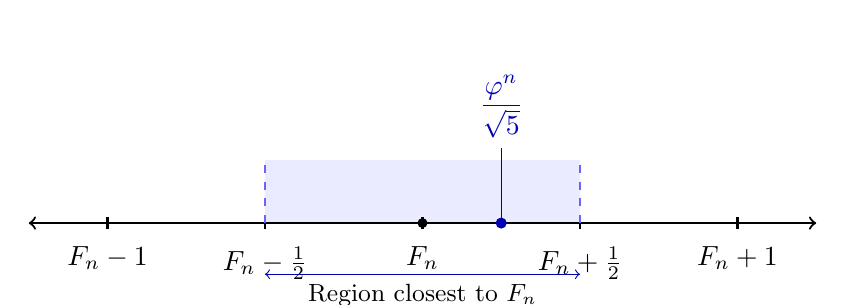
\begin{tikzpicture}[x=4cm, y=1cm]

        % Shaded region
        \fill[blue!8] (-0.5,0) rectangle (0.5,0.8);

        % Number line
        \draw[<->, thick] (-1.25,0) -- (1.25,0);

        % Tick marks and labels
        \foreach \x/\lab in {
            -1/{F_n-1},
            -0.5/{F_n-\frac{1}{2}},
            0/{F_n},
            0.5/{F_n+\frac{1}{2}},
            1/{F_n+1}
        }{
            \draw[thick] (\x,-0.08) -- (\x,0.08);
            \node[below=5pt] at (\x,0) {$\lab$};
        }

        % Boundaries
        \draw[dashed, blue!60] (-0.5,0) -- (-0.5,0.8);
        \draw[dashed, blue!60] (0.5,0) -- (0.5,0.8);

        % Fibonacci number
        \fill[black] (0,0) circle (1.8pt);

        % Expression (illustrative position)
        \fill[blue!70!black] (0.25,0) circle (2pt);
        \draw[blue!70!black] (0.25,0) -- (0.25,0.95);

        \node[above, blue!70!black] at (0.25,0.95)
            {$\dfrac{\varphi^n}{\sqrt{5}}$};

        % Interval annotation
        \draw[<->, blue!70!black]
            (-0.5,-0.65) -- (0.5,-0.65);

        \node[below, font=\small] at (0,-0.65)
            {Region closest to $F_n$};

    \end{tikzpicture}

    \caption{The expression $\varphi^n/\sqrt{5}$ always
    lies within half a unit of the integer $F_n$.
    Its position is illustrative.}
    \label{fig:closest-integer}
\end{figure}

Since the expression lies strictly within this interval,
no other integer can be closer to it than $F_n$.

Hence, $F_n$ is the closest integer to
$\varphi^n/\sqrt{5}$. \hfill $\square$


\subsection*{3.4 Numerical Illustration}

We can also illustrate the result numerically by
calculating the absolute error for different values of $n$.

Let
\[
E_n =
\left|\dfrac{\varphi^n}{\sqrt{5}} - F_n\right|
= \dfrac{|\psi|^n}{\sqrt{5}}
\]

\begin{table}[htbp]
    \centering
    \renewcommand{\arraystretch}{1.4}

    \begin{tabular}{rrrr}
        \toprule
        $n$ &
        $\dfrac{\varphi^n}{\sqrt{5}}$ &
        $F_n$ &
        Absolute Error ($E_n$) \\
        \midrule
         0 &    0.447214 &    0 & 0.447214 \\
         1 &    0.723607 &    1 & 0.276393 \\
         2 &    1.170820 &    1 & 0.170820 \\
         3 &    1.894427 &    2 & 0.105573 \\
         4 &    3.065248 &    3 & 0.065248 \\
         5 &    4.959675 &    5 & 0.040325 \\
        10 &   55.003636 &   55 & 0.003636 \\
        20 & 6765.000030 & 6765 & 0.000030 \\
        \bottomrule
    \end{tabular}

    \caption{Comparison of Fibonacci numbers with
    $\varphi^n/\sqrt{5}$.}
    \label{tab:fibonacci-error}
\end{table}


\begin{figure}[htbp]
    \centering

    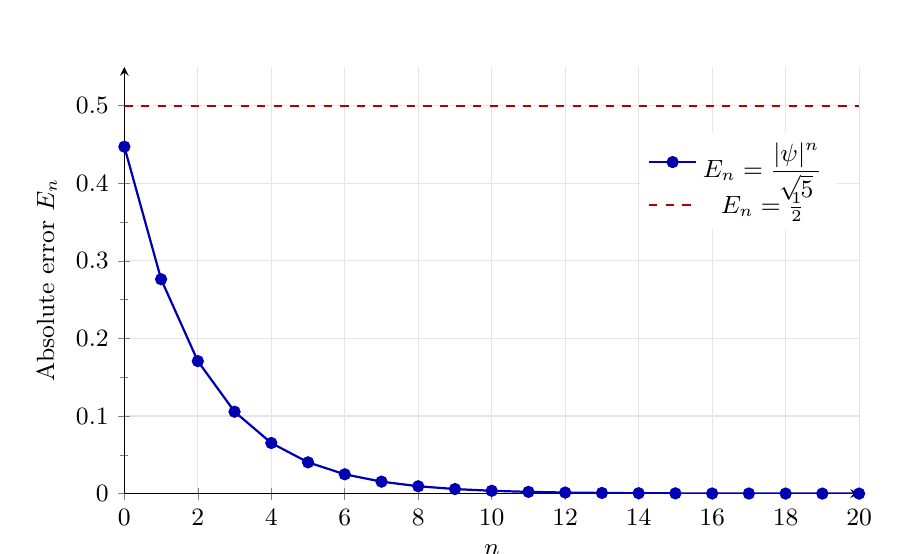
\begin{tikzpicture}
        \begin{axis}[
            width=0.9\textwidth,
            height=7cm,
            axis lines=left,
            xlabel={$n$},
            ylabel={Absolute error $E_n$},
            xmin=0,
            xmax=20,
            ymin=0,
            ymax=0.55,
            xtick={0,2,...,20},
            ytick={0,0.1,...,0.5},
            minor y tick num=1,
            grid=major,
            grid style={gray!20},
            tick label style={font=\small},
            label style={font=\small},
            legend style={
                at={(0.97,0.85)},
                anchor=north east,
                draw=none,
                font=\small
            }
        ]

        % Absolute error
        \addplot[
            blue!70!black,
            thick,
            mark=*,
            mark size=1.8pt,
            domain=0:20,
            samples=21
        ]
        {((sqrt(5)-1)/2)^x/sqrt(5)};

        \addlegendentry{
            $E_n=\dfrac{|\psi|^n}{\sqrt{5}}$
        }

        % Upper bound
        \addplot[
            red!70!black,
            dashed,
            thick,
            domain=0:20,
            samples=2
        ]
        {0.5};

        \addlegendentry{$E_n=\frac{1}{2}$}

        \end{axis}
    \end{tikzpicture}

    \caption{Exponential decay of the absolute error
    as $n$ increases.}
    \label{fig:fibonacci-error}
\end{figure}

The error decreases exponentially as $n$ increases
because $|\psi| < 1$.

This also gives us a remarkably compact way of expressing
Fibonacci numbers using the floor function:

\[
\boxed{
F_n =
\left\lfloor
\dfrac{\varphi^n}{\sqrt{5}} + \dfrac{1}{2}
\right\rfloor
}
\]
\end{document}